\begin{comment}
	\pagebreak
\end{comment}

\begin{comment}
	\textbf{Taxonomy of generative learning:}\\
	\textbf{Supervised learning:} Tries to learn a function that maps $X \Rightarrow Y$, used in classification, regression, object detection and segmentation.\\
	\textbf{Unsupervised Learning:} The Goal here is to learn the hidden structure of the data, such as in clustering, feature learning, dimensionality reduction or density estimation.\\
	\textbf{Generative Modeling (our Goal):} Given training data, learn a distribution and generate new samples drawn from the learned distribution.
	Learn $p_{model}$ close to $p_{data}$, generate from $p_{model}$\\
	\begin{Figure}
 		\centering
 		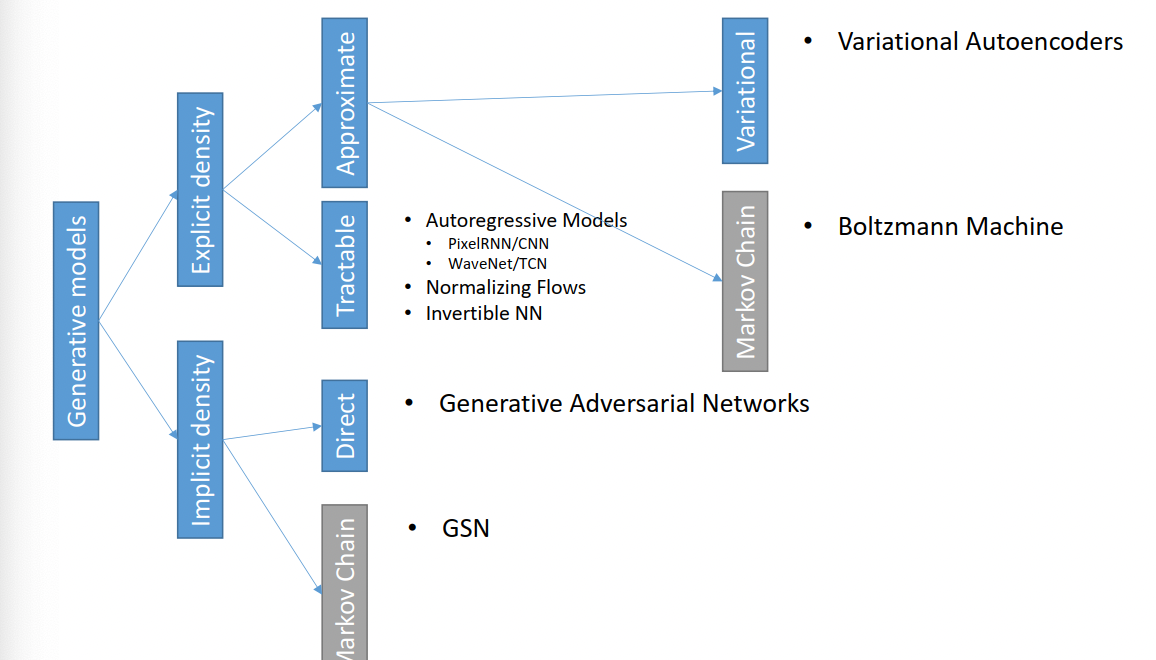
\includegraphics[width=\linewidth]{graphic/vae-taxonomy}
 		\captionof{figure}{Taxonomy of variational models}
	\end{Figure}
\end{comment}
\begin{Figure}
 		\centering
 		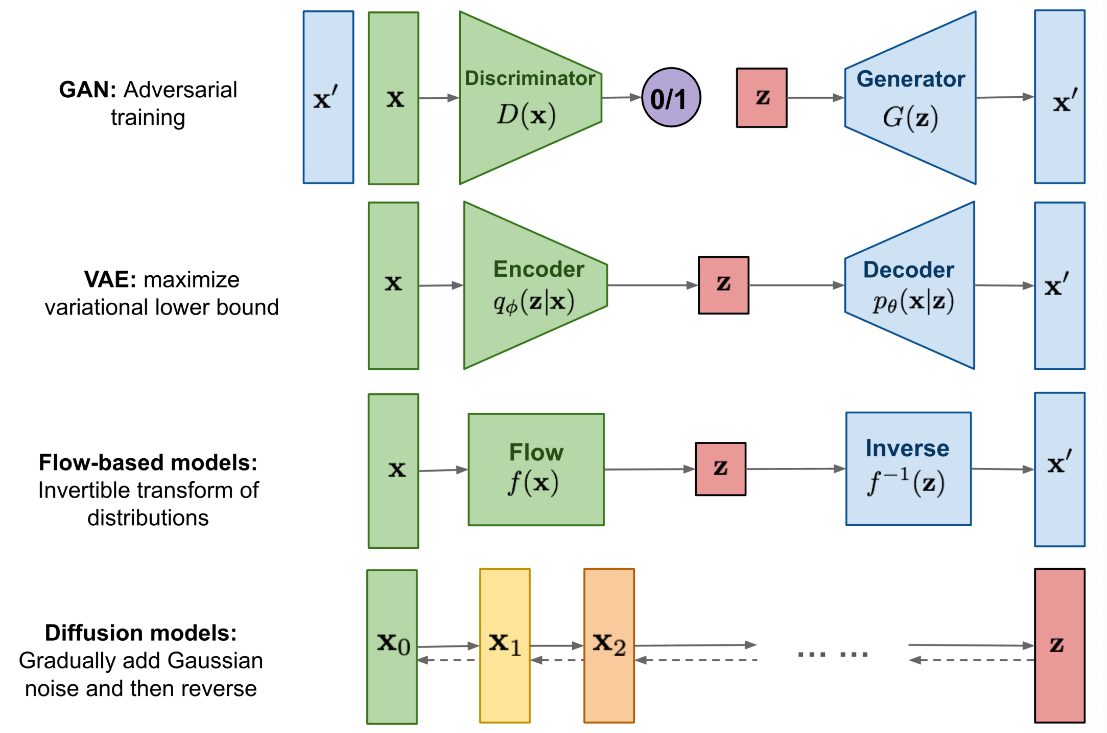
\includegraphics[width=\linewidth]{graphic/gen-overview}
\end{Figure}

\section{Variational Auto Encoders}
\begin{comment}
		\begin{Figure}
 		\centering
 		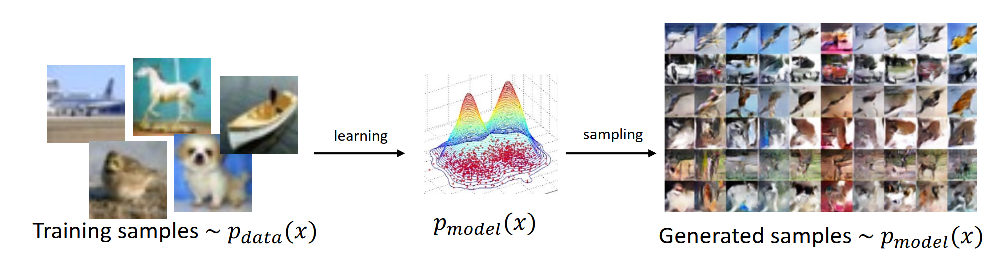
\includegraphics[width=\linewidth]{graphic/vae-example}
 		\captionof{figure}{VAE Pipeline}
	\end{Figure}
\end{comment}

\textbf{AE:} optimize $\theta_f, \theta_g = \argmin \sum_n^N \norm{x_n - g_\theta(f_\theta(x_n))} ^2$\\
\begin{comment}
	\textbf{The encoder} projects the original input to a latent space Z. 
	It has to figure out what are the important features worth keeping (f.e. when dim(Z) $<$ dim(X)).\\
	\textbf{The decoder} learns to construct an output from a sample of Z.\\ 
	In the optimal case, the encoder-decoder pipeline approximates the identity function of the data.\\

	\begin{Figure}
 		\centering
 		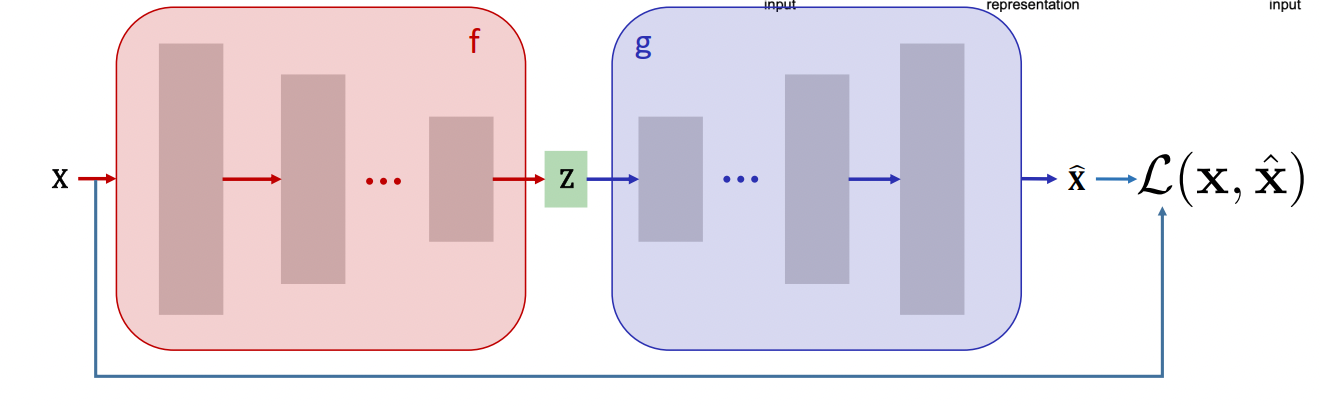
\includegraphics[width=\linewidth]{graphic/vae-ae-2}
 		\captionof{figure}{Auto-Encoders Model with loss}
	\end{Figure}
\end{comment}

\textbf{PCA:} $z = f(x) = Wx + b$, $\whx = g(z) = W^* z + c$\\
\begin{comment}
	linear embedding along the principle components.
\end{comment}

\textbf{NN:} $z = f(x) = \sigma(Wx + b)$, $\whx = g(\wha (x)) = \sigma(W^*z + c)$\\

\textbf{Latent Space:} meaningful DOF, continous and interpolatable\\
undercomp: compress, features; overcomp: copy components\\
\begin{comment}
	Not all DOF are important, when we look at the image space (f.e. 256 x 256 x 3), we could as well sample something very random which does not represent an image.\\
	\textbf{Undercomplete Z:} Compressed representation, learns important features of input. Bad for out-of-distribution samples\\
	\textbf{Overcomplete Z:} Hidden units copies input components, but might not extract meaningful structure.\\
	\begin{Figure}
 		\centering
 		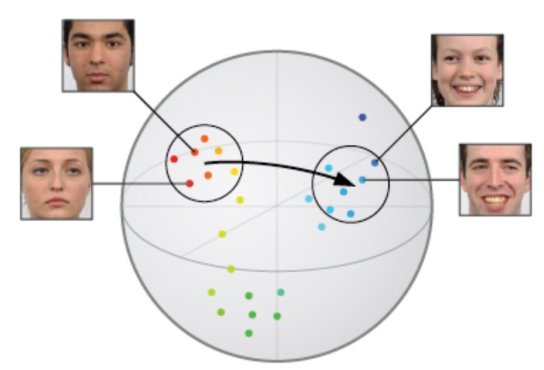
\includegraphics[width=\linewidth]{graphic/vae-latent-space}
 		\captionof{figure}{Latent space}
	\end{Figure}
\end{comment}


\textbf{Denoise:} input+gaussian noise, reconstruct w. overcomp. z\\
\begin{comment}
	\Note{The Latent space is overcomplet in this instance}\\
	The model learns components of the images, which it can add to the obstructed image in the end.
	
	\begin{Figure}
 		\centering
 		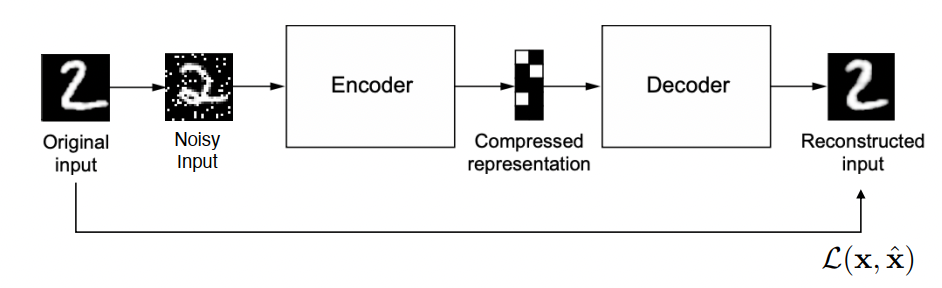
\includegraphics[width=\linewidth]{graphic/vae-denoising}
 		\captionof{figure}{VAE pipeline for denoising}
	\end{Figure}
	\begin{Figure}
 		\centering
 		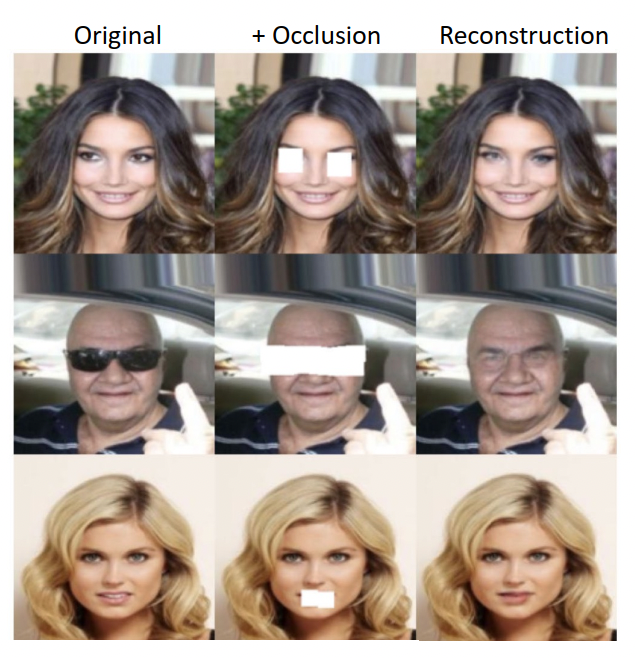
\includegraphics[width=\linewidth]{graphic/vae-denoising-ex}
 		\captionof{figure}{VAE de-noising example}
	\end{Figure}
\end{comment}


\textbf{Limit:} z not interpolatable; +reconstruction, -new samples\\
\begin{comment}
	Freshly generated samples from latent space Z do not make much sense, as in these regions, the decoder doesn't know what makes sense.
	Still, for reconstruction, the latent space is very good.
	
	\begin{Figure}
 		\centering
 		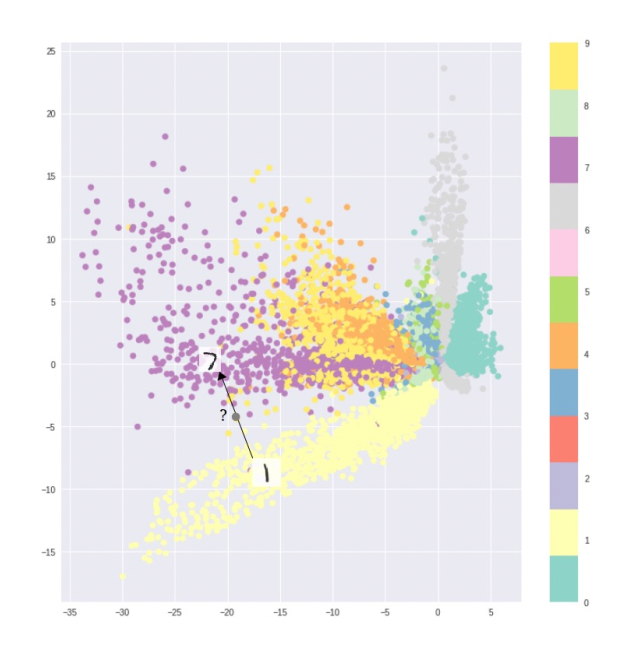
\includegraphics[width=0.7\linewidth]{graphic/vae-mnist-embedding}
 		\captionof{figure}{AE MNIST embedding, points in the space}
	\end{Figure}
\end{comment}

\textbf{VAE:} The latent space Z is approximated by $f(x) \sim \cN(\hat{\mu}, \hat{\sigma}I)$\\
\begin{comment}
	\begin{Figure}
 		\centering
 		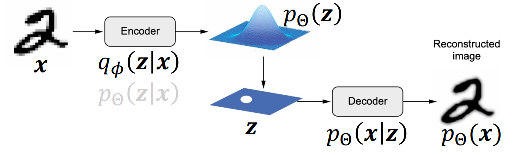
\includegraphics[width=\linewidth]{graphic/vae-distributions}
 		\captionof{figure}{VAE Learned distributions}
	\end{Figure}
	
	By design, the latent space is compact and interpolatable.
	This allows easy sampling and interpolation when generating new samples.
	
	\begin{Figure}
 		\centering
 		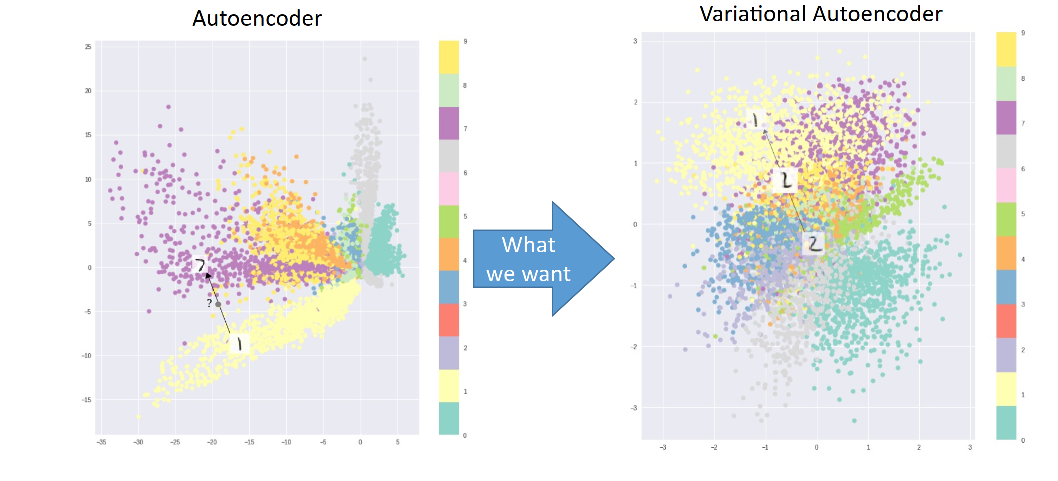
\includegraphics[width=\linewidth]{graphic/vae-latent-space-2}
 		\captionof{figure}{VAE Latent space}
	\end{Figure}
\end{comment}

\textbf{Encode:} $q_\phi(z|x)$ for $\mu_{(z|x)}, \Sigma_{(z|x)}$, $z|x \sim \cN(\mu_{(z|x)}, \Sigma_{(z|x)})$\\
\begin{comment}
	The Encoder outputs a vector each for $\mu, \sigma$.
	This multivariate gaussian can them be sampled to get the latent vector Z depending on x.\\
	\textbf{Problem:} Using only the reconstruction error (MSE), the variance is going to be reduced to zero and the individual classes form clusters around their means.
	This leads to bad interpolation performance.
	We want to force the encoder to find features that are as close as possible to each other, while still being distinct.
	
	\begin{Figure}
 		\centering
 		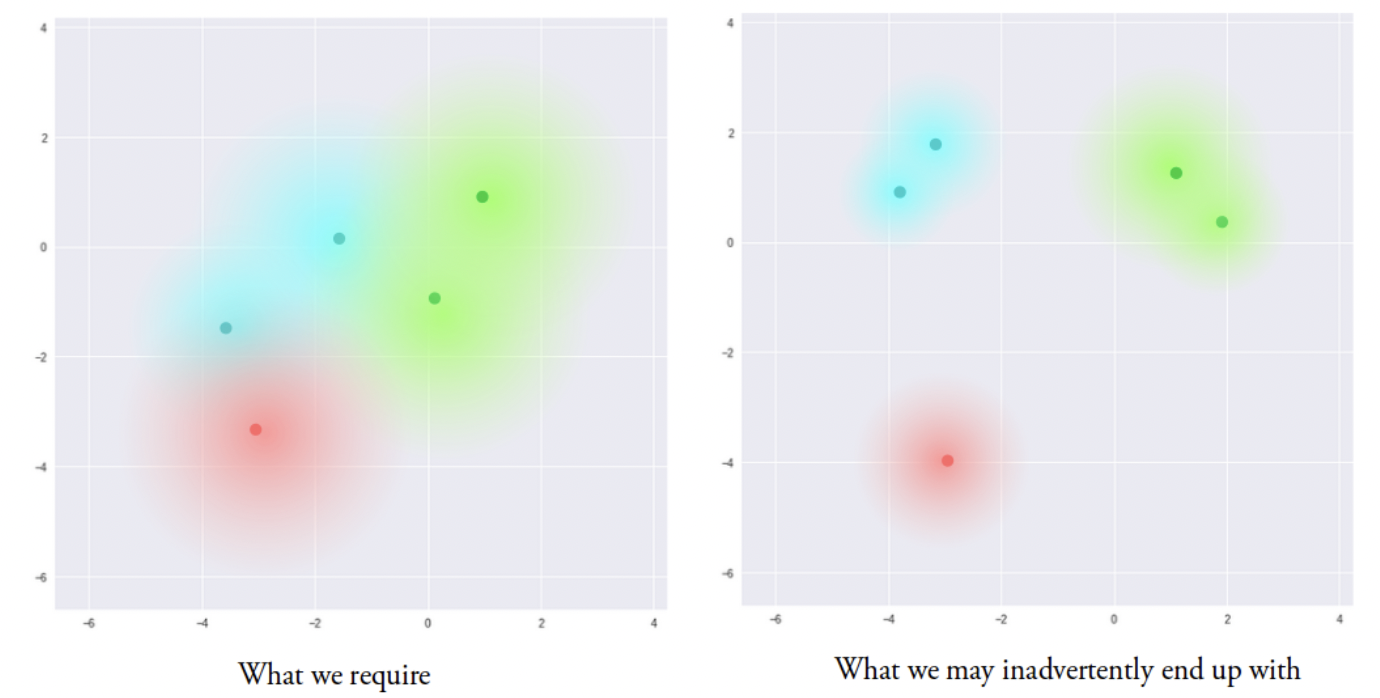
\includegraphics[width=\linewidth]{graphic/vae-encoder-challenge}
 		\captionof{figure}{VAE Reconstruction loss only}
	\end{Figure}
\end{comment}

\textbf{Decode:} $p_{\theta}(x|z)$ for $\mu_{(\whx|z)}, \Sigma_{(\whx|z)}$, $\whx|z \sim \cN(\mu_{(\whx|z)}, \Sigma_{(\whx|z)})$\\
LH: $p_\theta(x) = \int_z p_\theta(x|z) p_\theta(z) dz$, Post: $p_\theta(z|x) = \frac{p_\theta(X|Z) p_\theta(z)}{p_\theta(x)}$\\
\begin{comment}
	The decoder, i.e. the conditional $p(x|z)$ is usually a NN, because the output can be really complex, f.e. if we want the generate an image.\\
\end{comment}

\textbf{KL:} $-D_{KL}(q_\phi(z|x) || p_\theta(z)) = \int_x q_\phi(z|x) \log(\frac{p_\theta(z)}{q_\phi(z|x)})$\\
$= \frac{1}{2} \sum^J_i (1+ \log(\sigma_j^2) - \mu_j - \sigma_j^2),$ if $q \sim \cN(\mu, \sigma I), p \sim \cN(0,I)$\\
Properties: asymmetric and non-negative\\
\textit{from exercise:} $\int p(z) \log q(z)dz = \\
- \frac{J}{2} \log 2\pi - \frac{1}{2} \sum_i^J \log \sigma_{p,j} - \frac{1}{2} \sum_j^J \frac{\sigma^2_{p,j} + (\mu_{p,j} - \mu_{q,j})^2}{\sigma^2_{q,j}}$\\
\begin{comment}
	KL meassures how similar two distributions are.
	We punish the encoder if the final distribution diverges away from the standart normal.
	\Note{Assymetric and non-negative}\\
\end{comment}

\textbf{ELBO:} $p_\theta(x) \geq E_{q_\phi(z|x)}[\log p_\theta(x|z)] - D_{KL}(q_\phi(z|x) || p_\theta(z))$\\
\begin{comment}
	The first part of the loss is the reconstruction loss. 
	It meassures the loss from the decoder prediction.\\
	The second part of the loss is the latent code loss. 
	It enforces that the latent space is a gaussian, e.g. enforcing properties such as compactness and good interpolation\\
	\Note{We want to maximize the ELBO}\\
	\Note{If we have a sequence, the ELBO is the sum of all variational lower bounds}\\
	\Note{The different classes are still entangled, interpolation works good, but features are not distinguishing unique properties.}
	\begin{Figure}
 		\centering
 		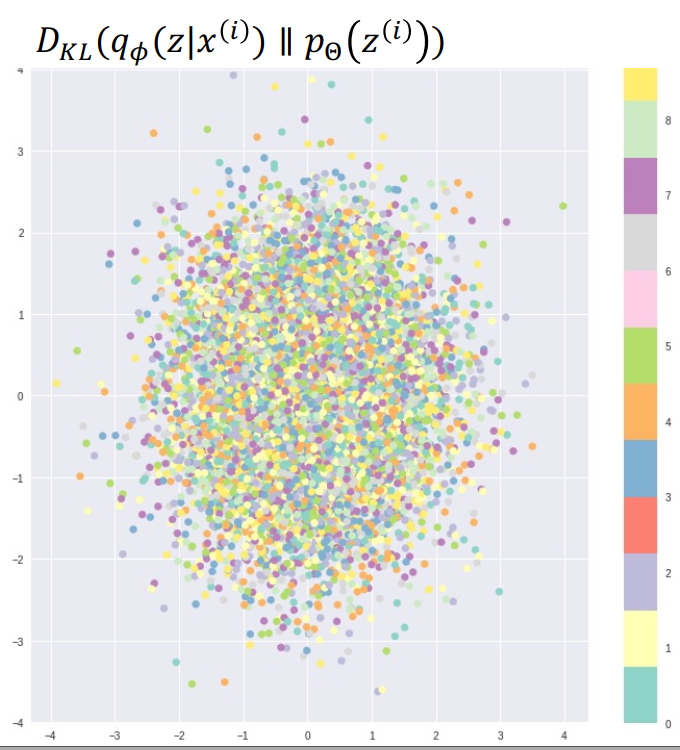
\includegraphics[width=0.4\linewidth]{graphic/vae-latent-space-loss}
 		 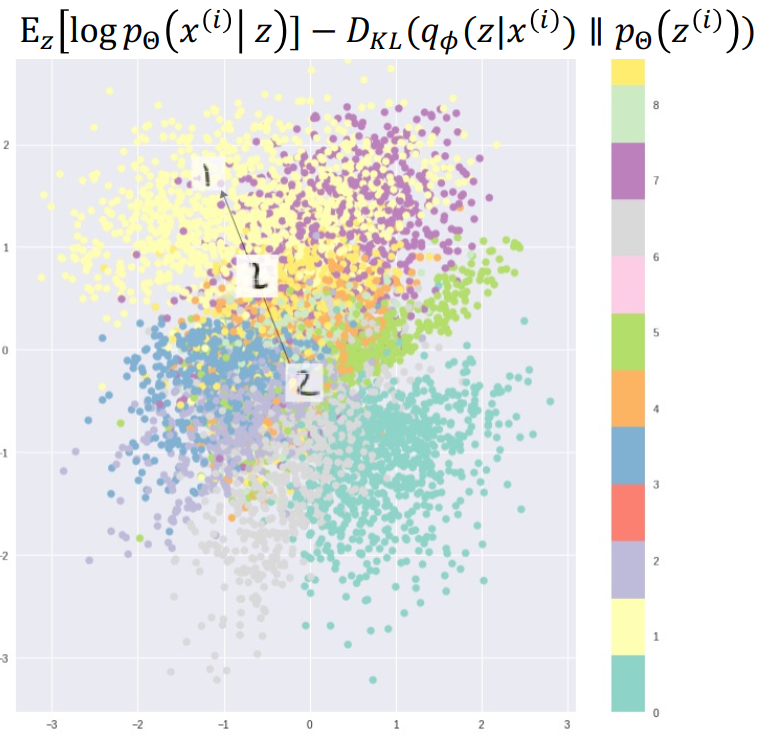
\includegraphics[width=0.4\linewidth]{graphic/vae-both-loss}
 		\captionof{figure}{VAE KL-Loss only vs. both losses (entangled)}
	\end{Figure}
\end{comment}

\textbf{Re-parameterization:} $z = \mu + \sigma \epsilon$, $\epsilon \sim \cN(0,1)$\\

\textbf{Goal:} Learn features that correspond to distinct factors of variaton e.g., digits and style (or thickness, orientation)
\begin{comment}
	Statistical independence of the of the features can be used\\
	In the picture below, one can see that the AE might achieve detangled features, but it is bad for interpolation. The KL divergence loss craetes some entaglement, though.\\
	\begin{Figure}
 		\centering
 		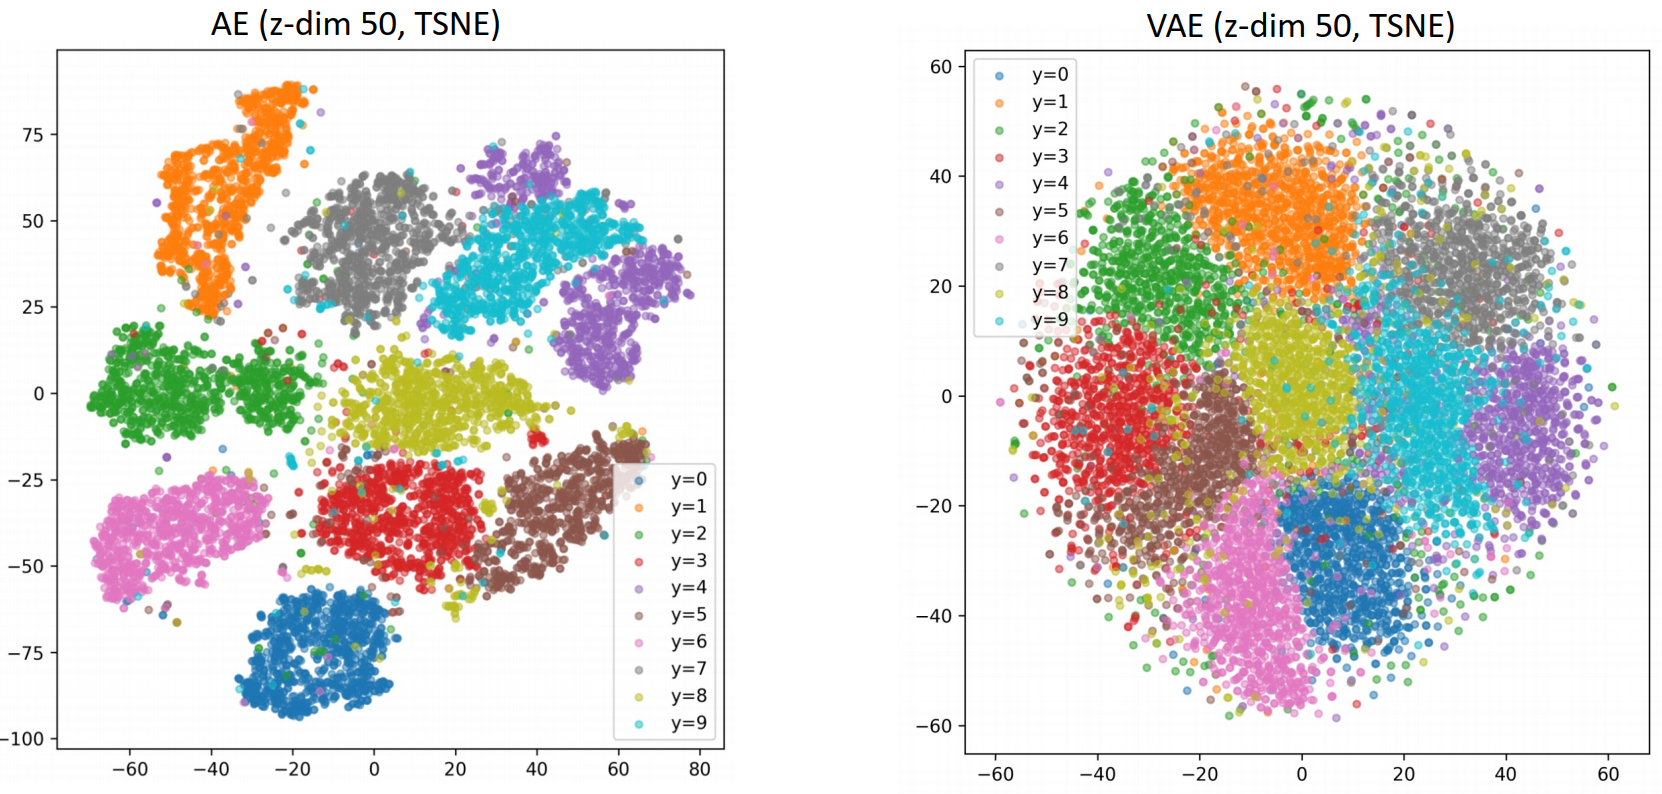
\includegraphics[width=\linewidth]{graphic/vae-regularization-entaglement}
 		\captionof{figure}{VAE vs. AE}
	\end{Figure}
\end{comment}

\textbf{$\beta$-VAE:} $\cL = -E_{q_\phi(z|x)}[\log p_\theta(x|z)] + \beta D_{KL}(q_\phi(z|x) || p_\theta(z))$\\
\begin{comment}
	\textbf{Goal} is to disentangle the different features.
	The KL-loss tries to create a diagonal multivariate Gaussian, which perfectly seperates the independent features.
	The reconstruction loss fucks this up, as it fights for the loss as well.\\
	Putting more weight for the KL loss helps solving it in an unsupervised fashion.
	Alternatively, could condition on features.
	
	\begin{Figure}
 		\centering
 		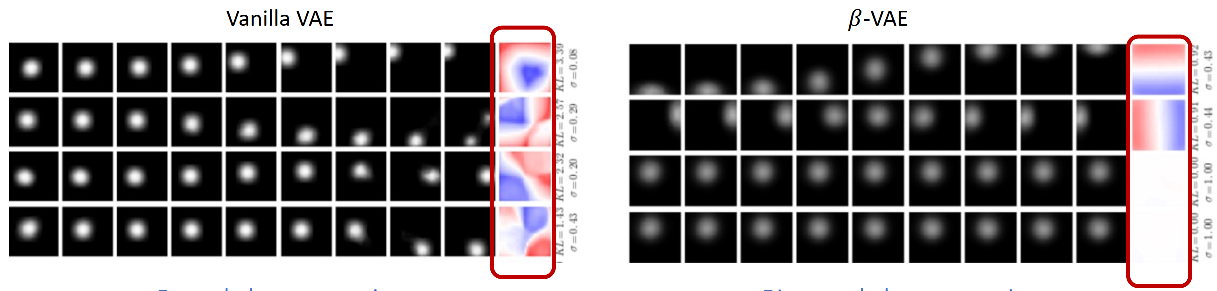
\includegraphics[width=\linewidth]{graphic/vae-disentangled}
 		\captionof{figure}{VAE Entangled vs. Disentangled representation}
	\end{Figure}
\end{comment}

\textbf{Faces:} generated faces are typically blurry\\












